\appendix

\chapter{Proofs}
\label{ch:proofs}
\section{Proof of Lemma~\ref{lemma:dual}}
\label{sec:prooflemmadual}

\renewcommand{\thetheorem}{4.\arabic{theorem}}

\begin{lemma}
	The dual problem of \eqref{eq:entropynew} is given by 
	\begin{equation*}
		D(\alpha, \beta) := \sum_{i=1}^m \alpha_i \mu_i + \sum_{j=1}^n \beta_j \nu_j - \varepsilon \sum_{i=1}^m \sum_{j=1}^n \exp\left(\frac{\alpha_i + \beta_j - c_{ij} - \varepsilon}{\varepsilon}\right),
		\tag{\ref{eq:Dinproof}}
	\end{equation*}
	and the dual optimization problem is given by 
	\begin{equation*}
		\max_{\alpha \in \R^m, \beta\in \R^n} D(\alpha, \beta).
		\tag{\ref{eq:dual}}
	\end{equation*}
\end{lemma}
\begin{proof}
	Consider equation~\eqref{eq:entropynew} and introduce the Lagrangian multipliers $\alpha \in \R^m, \beta\in \R^n$; $\alpha$ and $\beta$ penalize deviations from the marginal constraints. Now, at the optimum there should hold (by definition of Lagrangian multipliers)
	\begin{subequations}
		\begin{equation}
			g_1 (i) = \sum_{j=1}^n \pi_{ij} - \mu_i = 0,
		\end{equation}
		\begin{equation}
			g_2(j) =\sum_{i=1}^m \pi_{ij} - \nu_j = 0.
		\end{equation}
		\label{eq:g}
	\end{subequations}
	
	By definition of a Lagrangian multiplier, if we want to minimize $f(z)$ subject to $g(z) = 0$, we have 
	\begin{equation*}
		\L(z, \lambda) = f(z) \pm \kappa  g(z),
	\end{equation*}
	with $\L$ the Lagrangian, $\kappa$ the Lagrangian multiplier and the $\pm$ a convention. For simplicity, let us take the expression with $+$. Note that $\alpha$ and $\beta$ are incorporated in $\kappa$. Then, the Lagrangian is
	\begin{align*}
		\mathcal{L}(\pi, \alpha, \beta) = & \sum_{i=1}^m \sum_{j=1}^n \left[c_{ij} \pi_{ij} + \varepsilon \pi_{ij} \log(\pi_{ij})\right] \\
		& - \sum_{i=1}^m \alpha_i g_{1}(i) - \sum_{j=1}^n \beta_j g_{2}(j),
	\end{align*}
	with $g_{1}(i), g_{2}(j)$ as in \eqref{eq:g}. Expanding the terms with the multipliers gives us
	\begin{align*}
		- \sum_{i=1}^m \alpha_i \left[\sum_{j=1}^n \pi_{ij} - \mu_i \right] &= - \sum_{i=1}^m \sum_{j=1}^n \alpha_i \pi_{ij} + \sum_{i=1}^m \alpha_i \mu_i.
	\end{align*}
	Similarly,
	\begin{align*}
		- \sum_{j=1}^n \beta_j \left[\sum_{i=1}^m \pi_{ij} - \nu_j \right] &= - \sum_{i=1}^m \sum_{j=1}^n \beta_j \pi_{ij} + \sum_{j=1}^n \beta_j \nu_j.
	\end{align*}
	Thus, we see for the Lagrangian
	\begin{align}
		\mathcal{L}(\pi, \alpha, \beta) = & \sum_{i=1}^m \sum_{j=1}^n \left[c_{ij} \pi_{ij} + \varepsilon \pi_{ij} \log(\pi_{ij}) \right] \nonumber\\
		& - \sum_{i=1}^m \sum_{j=1}^n \alpha_i \pi_{ij} + \sum_{i=1}^m \alpha_i \mu_i  - \sum_{i=1}^m \sum_{j=1}^n \beta_j \pi_{ij} + \sum_{j=1}^n \beta_j \nu_j \nonumber \\
		= & \sum_{i=1}^m \sum_{j=1}^n \left[c_{ij} + \varepsilon \log(\pi_{ij}) - \alpha_i - \beta_j \right] \pi_{ij}  + \sum_{i=1}^m \alpha_i \mu_i + \sum_{j=1}^n \beta_j \nu_j. \label{eq:lagrangian}
	\end{align}
	Now, for the dual problem, we want to minimize $\L$ over $\pi$ for fixed $\alpha^*$ and $\beta^*$. Thus the minimum can be found by setting the partial derivative of $\mathcal{L}$ with respect to $\pi$ to zero:
	\begin{equation*}
		\frac{\partial 	\mathcal{L}(\pi^*, \alpha^*, \beta^*) }{\partial \pi^*_{ij}} = c^*_{ij} + \varepsilon \log(\pi_{ij}^*) - \alpha^*_i - \beta^*_j + \varepsilon  = 0.
	\end{equation*}
	Then, we can see
	\begin{equation*}
		-\varepsilon \log(\pi_{ij}^*) = c^*_{ij} - \alpha^*_i - \beta^*_j + \varepsilon,
	\end{equation*}
	thus
	\begin{equation}
		\pi_{ij}^* = \exp\left(\frac{\alpha_i^* + \beta_j^* - c_{ij}^* - \varepsilon}{\varepsilon}\right).
		\label{eq:rhodef}
	\end{equation}
	Therefore, we can see
	\begin{align*}
		\mathcal{L}(\pi, \alpha, \beta)& - \sum_{i=1}^m \alpha_i \mu_i - \sum_{j=1}^n \beta_j \nu_j \\
		=& \sum_{i=1}^m \sum_{j=1}^n \left[c_{ij} + \varepsilon \log(\pi_{ij}) - \alpha_i - \beta_j \right] \pi_{ij} \\
		=&  \sum_{i=1}^m \sum_{j=1}^n \left[c_{ij} + \varepsilon \log\exp\left(\frac{\alpha_i + \beta_j - c_{ij} - \varepsilon}{\varepsilon}\right) - \alpha_i - \beta_j \right] \pi_{ij} \\
		=& -\varepsilon \sum_{i=1}^m \sum_{j=1}^n \exp\left(\frac{\alpha_i + \beta_j - c_{ij} - \varepsilon}{\varepsilon}\right).
	\end{align*}
	Thus, the dual problem is given by
	\begin{equation*}
		D(\alpha, \beta) := \sum_{i=1}^m \alpha_i \mu_i + \sum_{j=1}^n \beta_j \nu_j - \varepsilon \sum_{i=1}^m \sum_{j=1}^n \exp\left(\frac{\alpha_i + \beta_j - c_{ij} - \varepsilon}{\varepsilon}\right),
	\end{equation*}
	and the dual optimization problem is given by
	\begin{equation*}
		\max_{\alpha \in \R^m, \beta\in \R^n} D(\alpha, \beta).
	\end{equation*}
\end{proof}

\section{Proof of Theorem~\ref{thm:2}}
\label{sec:proofthm2}
\begin{theorem}
	The optimization problem in equations~\eqref{eq:KLa} and \eqref{eq:KLb} is equivalent to 
	\begin{equation}
			\min _{\alpha \in \R^m, \beta \in \R^n, c\in \R^{m \times n}} E(\alpha, \beta, c)+R(c), \tag{\ref{eq:10}} 
	\end{equation}
	with 
	\begin{equation}
		E(\alpha, \beta, c) := \sum_{i,j} c_{ij} \pihat_{ij} - \sum_i \alpha_i \mu_i - \sum_j \beta_j \nu_j + \varepsilon \sum_{i,j} e^{(\alpha_i + \beta_j - c_{ij}-\varepsilon)/\varepsilon} . \tag{\ref{eq:E}}
	\end{equation}
	Here, equivalent means that $c^*$ solves \eqref{eq:KL} if and only if $(\alpha^{c^*}, \beta^{c^*}, c^*)$ solves \eqref{eq:10} with $(\alpha^{c^*}, \beta^{c^*})$ the optimal solution for the dual problem \eqref{eq:dual} with cost $c^*$.
\end{theorem}
\begin{proof}
	Recall from the proof of Lemma~\ref{lemma:dual}, equation~\eqref{eq:rhodef}, that the optimal transport plan is given by
	\[ \pi_{ij}^* = \exp\left[\f{\alpha_i^* + \beta_j^* - c_{ij}^* - \varepsilon}{\varepsilon}\right] . \]
	Note that $\pi^c_{ij} > 0$ for all $i,j$. Now, we can see 
	\begin{align}
		\chat = \text{KL}(\pihat, \pi^c) =  \sum_{i,j} \pihat_{ij} \log\left(\f{\pihat_{ij}}{\pi_{ij}^*}\right)\nonumber \\
		= & \sum_{i,j} \pihat_{ij} \left[\log\left(\pihat_{ij}\right) - \log\left(\pi_{ij}^*\right)\right] \nonumber\\
		= & -H(\pihat) - \f{1}{\varepsilon} \sum_{i,j} \pihat_{ij} (\alpha_i^* + \beta_j^* - c_{ij}^*-\varepsilon),
		\label{eq:KLinproof}
	\end{align}
	with $H$ as in equation~\eqref{eq:entropyH}, and $\pihat$ as in \eqref{eq:pi}. Note that since $\mu$ and $\nu$ are marginals of $\pi$, we can see 
	\begin{equation}
		\sum_{i,j} \alpha_{i}\pi_{ij}= \sum_i \alpha_i \mu_i, \quad \sum_{i,j} \beta_{j}\pi_{ij}= \sum_i \beta_j \nu_j.
		\label{eq:marginals}
	\end{equation}
	Then, plugging \eqref{eq:rhodef} and \eqref{eq:KLinproof} into \eqref{eq:KLa}, we can find
	\begin{align}
		\chat = &\min_c\; \text{KL}(\pihat, \pi^c) + \varepsilon^{-1} R(c)  \nonumber \\
		= & \min_c \left[\sum_{i,j} \pihat_{ij} \left(\log(\pihat_{ij}) - \log(\pi^c_{ij})\right) \varepsilon^{-1} R(c) \right] \nonumber \\
		= & \min_c \left[\sum_{i,j} \pihat_{ij}\log(\pihat_{ij}) - \sum_{i,j} \pihat_{ij} \f{\alpha_i + \beta_j - c_{ij} - \varepsilon}{\varepsilon} - \varepsilon^{-1} R(c) \right] \nonumber \\
		= & \min_c \left[H(\pihat) - \varepsilon^{-1}\left(\sum_{i,j} \pihat_{ij} \left(\alpha_i + \beta_j - c_{ij} - \varepsilon\right) -  R(c) \right) \right] \nonumber \\
		= & \min_c \left[ - \sum_i \alpha_i \mu_i - \sum_j \beta_j \nu_j +  \sum_{i,j} c_{ij} \pihat_{ij} +  R(c) \right],
		\label{eq:minimization}
	\end{align}
	where, in the last step we used equation~\eqref{eq:marginals}, and the fact that since $H(\pihat)$ is independent of $c$ and thus does not alter the minimization, and so does multiplication by some constant $\varepsilon > 0$ or addition of a scalar ($\varepsilon \sum_{i,j} \pihat_{ij}  = \varepsilon$). \par 
	Now, plugging this into \eqref{eq:E}, we can see
	\begin{align}
		E(\alpha^*, \beta^*, c^*) := & \sum_{i,j} c_{ij}^* \pihat_{ij} - \sum_i \alpha_i^* \mu_i - \sum_j \beta_j^* \nu_j + \varepsilon \sum_{i,j} e^{(\alpha_i^* + \beta_j^* - c_{ij}^*-\varepsilon)/\varepsilon} \nonumber\\
		= & \sum_{i,j} c_{ij}^* \pihat_{ij} - \sum_i \alpha_i^* \mu_i - \sum_j \beta_j^* \nu_j + \varepsilon ,
		\label{eq:E2}
	\end{align}
	since 
	\begin{equation*}
		\sum_{i,j} e^{(\alpha^*_i + \beta^*_j - c_{ij}^*-\varepsilon)/\varepsilon} = \sum_{i,j} \pihat_{ij} = 1,
	\end{equation*}
	since $\pihat$ is a probability vector. Note again that adding a constant factor does not alter the minimization. However, since by assumption $(\alpha^c, \beta^c)$ is optimal for any fixed $c$ in the dual problem \eqref{eq:dual}, we can see 
	\begin{equation*}
		E(\alpha^c, \beta^c, c) = \min_{\alpha\in\R^m, \beta \in \R^n} E(\alpha, \beta, c).
	\end{equation*}
	Thus, we can see that equation~\ref{eq:KLb} has the same set of solutions as equation~\eqref{eq:E}. Now, if we combine this with equation~\eqref{eq:E2}, and eliminate $\varepsilon$, we find 
	\begin{equation*}
		\min _{\alpha\in\R^m, \beta \in \R^n, c\in \R^{m \times n}} E(\alpha, \beta, c)+R(c), 
	\end{equation*}
	which is exactly \eqref{eq:10}, as we wanted. \par 
\end{proof}

\section{Proof of Theorem~\ref{thm:3}} 
\label{sec:proofthm3}
\setcounter{theorem}{3}
\begin{theorem}
	The following statements are true for $E(\alpha, \beta, c)$ in \eqref{eq:10}:
	\begin{enumerate}[label=(\roman*)]
		\item $E(\alpha, \beta, c)$ is jointly convex in $(\alpha, \beta, c)$;
		\item $E$ is a constant on the equivalence class $[(\alpha, \beta, c)]$ for each $(\alpha, \beta, c) \in \W$; 
		\item The functional $\widetilde{E}: \widetilde{\W} \ra \R$ with $\widetilde{E}([(\alpha, \beta, c)]) = E(\alpha, \beta, c)$ is well defined;
		\item If $(\alpha^*, \beta^*, c^*)$ is a solution of \eqref{eq:10}, then the optimal transport plan $\pi^*$ in \eqref{eq:KL} is given by 
		\[\pi^*_{ij} = e^{(\alpha^*_i + \beta^*_j - c^*_{ij}-\varepsilon)/\varepsilon};\]
		\item $[(\alpha^*, \beta^*, c^*)]$ as in $(iv)$ is the unique minimizer of $\widetilde{E}$. 
	\end{enumerate}
\end{theorem}
\begin{proof}
	\begin{enumerate}[label=(\roman*)]
		\item \textit{$E(\alpha, \beta, c)$ is jointly convex in $(\alpha, \beta, c)$} : \\
		Let us define $\phi = (\alpha, \beta, c)$, $\psi = (\delta \alpha, \delta \beta, \delta c)$ and 
		\begin{equation*}
			f(\upsilon) := E(\phi + \upsilon \psi), 
		\end{equation*}	
		for $\upsilon \in \R$. Then, we can see, by filling in \eqref{eq:E},
		\begin{equation*}
			f(\upsilon) =  \sum_{i,j} (c_{ij} + \upsilon \delta c_{ij})\pihat_{ij} - \sum_i (\alpha_{i} + \upsilon \delta \alpha_{i}) \mu_i - \sum_j (\beta_{i} + \upsilon \delta \beta_{j}) \nu_j + \varepsilon \sum_{i,j} e^{(K_{ij} + \upsilon \Delta K_{ij}-\varepsilon)/\varepsilon},
		\end{equation*}
		with $K_{ij} := \alpha_i + \beta_j - c_{ij}$ and $\Delta K_{ij} := \delta \alpha_i + \delta \beta_j - \delta c_{ij}$. Then, we find for the derivative with respect to $\upsilon$:
		\begin{align*}
			f'(\upsilon) = &  \sum_{i,j} \delta c_{ij}\pihat_{ij} - \sum_i \delta \alpha_{i} \mu_i - \sum_j  \delta \beta_{j} \nu_j + \varepsilon \sum_{i,j} e^{(K_{ij} + \upsilon \Delta K_{ij}-\varepsilon)/\varepsilon} \left(\f{\Delta K_{ij}}{\varepsilon}\right)  \\
			= &  \sum_{i,j} \delta c_{ij}\pihat_{ij} - \sum_i \delta \alpha_{i} \mu_i - \sum_j  \delta \beta_{j} \nu_j +  \sum_{i,j} e^{(K_{ij} + \upsilon \Delta K_{ij}-\varepsilon)/\varepsilon} \Delta K_{ij}.
		\end{align*}
		And, for the second derivative:
		\begin{align*}
			f''(\upsilon) = & \sum_{i,j} e^{(K_{ij} + \upsilon \Delta K_{ij}-\varepsilon)/\varepsilon} \Delta K_{ij}  \left(\f{\Delta K_{ij}}{\varepsilon}\right) \\
			=& \f{1}{\varepsilon} \sum_{i,j} e^{(K_{ij} + \upsilon \Delta K_{ij}-\varepsilon)/\varepsilon} (\Delta K_{ij})^2 \geq 0.
		\end{align*}
		Thus, we can see that $E$ is jointly convex in $(\alpha, \beta, c)$. 
		
		\item \textit{$E$ is constant on each equivalence class $[(\alpha, \beta, c)]$}: \\
		Suppose $(\alpha, \beta, c) \sim (\bar{\alpha}, \bar{\beta}, \bar{c})$, and denote $\delta_{\alpha_i} := \alpha_i - \bar{\alpha}_i$ and $\delta_{\beta_j} := \beta_j - \bar{\beta}_j$. Then, we can see
		\[ \bar{c}_{ij} =\bar{\alpha}_i +\bar{\beta}_j -\alpha_i -\beta_j +c_{ij} = -\delta_{\alpha_i}-\delta_{\beta_j} + c_{ij}. \]
		Hence, we have
		\begin{align*}
		E(\bar{\alpha}, \bar{\beta}, \bar{c}) = & \sum_{i,j} \bar{c}_{ij} \pihat_{ij} - \sum_i \bar{\alpha}_i \mu_i - \sum_j \bar{\beta}_j \nu_j + \varepsilon \sum_{i,j} e^{(\bar{\alpha}_i + \bar{\beta}_j - \bar{c}_{ij} - \varepsilon)/\varepsilon} \\
			=& \sum_{i,j} (-\delta_{\alpha_i} - \delta_{\beta_j} + c_{ij}) \pihat_{ij} - \sum_i (\alpha_i - \delta_{\alpha_i}) \mu_i - \sum_j (\beta_j - \delta_{\beta_j}) \nu_j \\
			& + \varepsilon \sum_{i,j} e^{(\alpha_i + \beta_j - c_{ij} - \varepsilon)/\varepsilon}  \\
			=& E(\alpha, \beta, c) - \sum_i \delta_{\alpha_i} \left(\sum_j \pihat_{ij}\right) - \sum_j \delta_{\beta_j} \left(\sum_i \pihat_{ij}\right) + \sum_i \delta_{\alpha_i} \mu_i + \sum_j \delta_{\beta_j} \nu_j\\
			 =& E(\alpha, \beta, c) - \sum_i \delta_{\alpha_i} \mu_i - \sum_j \delta_{\beta_j} \nu_j + \sum_i \delta_{\alpha_i} \mu_i + \sum_j \delta_{\beta_j} \nu_j \\
			=& E(\alpha, \beta, c).
		\end{align*}
		where in the third step, we used the fact that $\mu, \nu$ are marginals of $\pi$. Thus $E$ is a constant on $[(\alpha, \beta, c)]$. 
		
		\item \textit{$\quad \widetilde{E}: \widetilde{\mathcal{W}} \rightarrow \mathbb{R}$ with $\widetilde{E}([(\alpha, \beta, c)])=E(\alpha, \beta, c)$ is well-defined}:\\
		As an immediate result of $(i i)$, we can set $\widetilde{E}: \widetilde{\mathcal{W}} \rightarrow \mathbb{R}$ as $\widetilde{E}([\phi]):=E(\phi)$ for every $[\phi] \in \widetilde{\mathcal{W}}$, then $\widetilde{E}$ is well-defined.
		
		\item \textit{The optimal transport plan $\pi^{*}$ is given by $\pi^{*}=e^{\left(\alpha^{*}+\beta^{*}-c^{*}-\varepsilon\right) / \varepsilon} $:}\\
		Let $(\alpha^*, \beta^*, c^*)$ be a minimizer of \eqref{eq:10}. Then, $(\alpha^*, \beta^*)$ minimizes $E(\alpha, \beta, c)$ if $c = c^*$. Thus, we find 
		\begin{align*}
			(\alpha^*, \beta^*) = & \argmin_{\alpha, \beta} E(\alpha, \beta, c^*) \\ 
			= & \argmin_{\alpha, \beta} \left\{ \varepsilon \sum_{i,j} e^{(\alpha_i + \beta_j - c_{ij}-\varepsilon)/\varepsilon} - \sum_i \alpha_i \mu_i - \sum_j \beta_j \nu_j \right\},
		\end{align*}
		where we can neglect the $c$-terms, as we assumed $c = c^*$ constant. \par 
		Hence, $(\alpha^*, \beta^*)$ is the optimal dual variable, thus the optimal transport plan is (from the same derivation as Lemma~\ref{lemma:dual}) 
		\[\pi^* = e^{(\alpha^* + \beta^* - c^*-\varepsilon)/\varepsilon} . \]
		
		\item \textit{$\left[\left(\alpha^{*}, \beta^{*}, c^{*}\right)\right]$ is the unique minimizer of $\widetilde{E}$}:\\
		Let $[\phi] = [(\alpha, \beta, c)], [\psi] = [(\delta \alpha, \delta \beta, \delta c)] \in \widetilde{W}$ be two distinct equivalence classes. Thus there is at least one pair $(i,j) \in X \times Y$ such that $\Delta K_{ij} := \delta\alpha_i + \delta\beta_j - \delta c_{ij} \neq 0$. \par 		
		Consider the function $\widetilde{f}(\upsilon) := \widetilde{E}([\phi + \upsilon \psi]) = E(\phi + \upsilon \psi)$. Then, in similar fashion as in $(i)$, its second derivative is:
		\[f''(\upsilon) = \frac{1}{\varepsilon} \sum_{i=1}^m \sum_{j=1}^n e^{(K_{ij} + \upsilon \Delta K_{ij})/\varepsilon} (\Delta K_{ij})^2 > 0,\]
		since $[\psi] \neq [0]$. Since we chose $[\phi]$ arbitrary, we can see $\widetilde{f}$ is strictly convex at every $[\phi] \in \widetilde{\W}$, thus $[\phi]$ is th unique minimizer of $\widetilde{E}$ on $\widetilde{\W}$. 
	\end{enumerate}
\end{proof}

\section{Proof of Lemma~\ref{lemma:inverseOT}}
\label{sec:prooflemmainverseOT}
\begin{lemma}
	The inverse Optimal Transport minimization \eqref{eq:10} has the same set of solutions as the following minimization:
	\begin{equation}
		\min _{\alpha, \beta, c} \Psi(\alpha, \beta, c):=F(\alpha, \beta, c)+R(c) , \tag{\ref{eq:lemma}}
	\end{equation}
	with
	\[ F(\alpha, \beta, c)=-\langle\alpha, \mu\rangle-\langle\beta, \nu\rangle+\langle c, \hat{\pi}\rangle+\varepsilon \log \left(\left\langle e^{\left(\alpha_{i}+\beta_{j}-c_{i j}-\varepsilon\right) / \varepsilon}, 1\right\rangle\right) .\]
\end{lemma}
\begin{proof} 
	%Observe that $s(\alpha, \beta, c)>0$ for all $(\alpha, \beta, c)$, with $s$ as in equation~\eqref{eq:s}. %Furthermore, we know log is strictly increasing on $(0, \infty)$. Therefore, we can see
	%\[ s(\alpha, \beta, c)=s\left(\alpha^{\prime}, \beta^{\prime}, c^{\prime}\right) \Leftrightarrow \log s(\alpha, \beta, c)=\log \left(\alpha^{\prime}, \beta^{\prime}, c^{\prime}\right) .\] 
	%for all $\alpha, \alpha^{\prime}\in \R^m, \beta, \beta^{\prime} \in \mathbb{R}^{n}$ and $c, c^{\prime} \in \R^{m \times n}$. The other parts of the equation remains the same as equation~\eqref{eq:10}. \par 
	Consider the minimization problem of \eqref{eq:lagrangian}
	\begin{equation*}
		\inf_{\sum_{i,j} \pi_{ij} = 1, \pi_{ij}\geq 0} \left\{ \sum_{i,j} \sigma_{ij}\pi_{ij} - \varepsilon \sum_{i,j} \pi_{ij} \log \pi_{ij} + \sum_i \alpha_i \mu_i + \sum_j \nu_j \beta_j \right\},
	\end{equation*}
	with $\sigma_{ij} = -\alpha_i -\beta_j + c_{ij}$. Then we get from equation~\eqref{eq:lagrangian} with the extra constraint $\sum_{i,j} \pi_{ij}= 1$ with associated Lagrangian multiplier $\lambda$: 
	\begin{equation*}
		\mathcal{L} (\pi, \alpha, \beta) = \sum_{i,j} \left[\pi_{ij} \sigma_{ij} + \varepsilon \pi_{ij} \log \pi_{ij}\right] + \lambda\left(\sum_{i,j} \pi_{ij} - 1\right) + \langle \alpha, \mu\rangle + \langle \beta, \nu \rangle. 
	\end{equation*}
	Differentiating this with respect to $\pi_{ij}$ gives us 
	\begin{equation*}
		\f{\del \mathcal{L}(\pi, \alpha, \beta)}{\del \pi_{ij}} = \sigma_{ij} + \varepsilon \log \pi_{ij} + \varepsilon - \lambda. 
	\end{equation*}
	Setting this derivative to zero at to minimize with respect to $\pi$, we get 
	\begin{equation}
		 \log \pi_{ij} =\exp\left( \f{-\sigma_{ij} - \varepsilon + \lambda}{\varepsilon}\right).
		 \label{eq:logpi}
	\end{equation}
	Then, with the additional constraint $\sum_{i,j} \pi_{ij}= 1$, we get 
	\begin{equation*}
		\sum_{i,j} \exp\left( \f{-\sigma_{ij} - \varepsilon + \lambda}{\varepsilon}\right) = 1,
	\end{equation*}
	so, since $\lambda$ and $\varepsilon$ are independent of $i$ and $j$:
	\begin{align*}
		\exp\left(\f{\lambda}{\varepsilon}\right) \sum_{i,j} \exp\left(\f{-\sigma_{ij} - \varepsilon}{\varepsilon}\right) = 1 \\
		\Rightarrow \lambda  = -\varepsilon \log \sum_{i,j} \exp \left(\f{-\sigma_{ij} - \varepsilon }{\varepsilon}\right) . 
	\end{align*}
	With this definition of $\lambda$ and filling in equation~\eqref{eq:logpi}, we can see
	\begin{align*}
		\sum_{i,j}& \sigma_{ij} \pi_{ij} + \varepsilon \sum_{i,j} \pi_{ij}\log \pi_{ij} \\ 
		= & \sum_{i,j} \sigma_{ij} \pi_{ij} + \varepsilon \sum_{i,j} \pi_{ij}\left(\f{-\sigma_{ij} - \varepsilon + \lambda}{\varepsilon}\right) \\
		= & \sum_{i,j}\sigma_{ij} \pi_{ij} - \sum_{i,j}\sigma_{ij} \pi_{ij} - \varepsilon \sum_{i,j}\pi_{ij} + \lambda \sum_{i,j} \pi_{ij} \\ 
		= & -\varepsilon + \lambda  \\ 
		= & -\varepsilon \log \sum_{i,j} \exp \left(\f{-\sigma_{ij} - \varepsilon}{\varepsilon}\right) - \varepsilon. 
	\end{align*}
	Thus, together with equation~\eqref{eq:lagrangian}, we can see for the dual problem of the entropy regularized OT with the extra constraint $\sum_{i,j} \pi_{ij} = 1$:
	\begin{equation*}
		\max_{\alpha \in \R^m, \beta\in \R^n} \langle \alpha, \mu \rangle + \langle \beta, \nu \rangle -\varepsilon \log \sum_{i,j} \exp \left(\f{\alpha_i + \beta_j - c_{ij} - \varepsilon }{\varepsilon}\right) - \varepsilon. 
	\end{equation*}
	For convenience, let us call 
	\begin{equation}
		D_2 (\alpha, \beta) := \langle \alpha, \mu \rangle + \langle \beta, \nu \rangle -\varepsilon \log \sum_{i,j} \exp \left(\f{\alpha_i + \beta_j - c_{ij} - \varepsilon }{\varepsilon}\right) - \varepsilon,
	\end{equation}
	and $D_1$ as $D$ as in equation~\eqref{eq:Dinproof}: 
	\begin{equation}
		D_1 (\alpha, \beta) := \langle \alpha, \mu \rangle + \langle \beta, \nu \rangle -\varepsilon \sum_{i,j} \exp \left(\f{\alpha_i + \beta_j - c_{ij} - \varepsilon }{\varepsilon}\right).
	\end{equation}
	Furthermore, let us call 
	\begin{align*}
		&A(\alpha, \beta) := \langle \alpha, \beta \rangle + \langle \beta, \nu \rangle, \\ &Z (\alpha, \beta, c) := \sum_{i,j} \exp \left(\f{\alpha_i + \beta_j - c_{ij} - \varepsilon }{\varepsilon}\right).
	\end{align*}
	Then, we can see 
	\begin{align*}
		&D_1 = A - \varepsilon Z,\\ &D_2 = A - \varepsilon \log Z - \varepsilon, 
	\end{align*}
	so 
	\[D_2 = D_1 + \varepsilon Z - \varepsilon \log Z - \varepsilon,\]
	and call 
	\[h(Z) := \varepsilon Z - \varepsilon \log Z - \varepsilon. \]
	Note that $D_1 = D_2$ if and only if $Z = 1$. We will show that at the optimal value $(\alpha^*, \beta^*)$, there holds $Z=1$. We can see 
	\begin{align*}
		\f{\del D_1}{\del \alpha_i}(\alpha^*, \beta^*) = & \mu_i - \sum_j \exp \left(\f{\alpha_i^* + \beta_j^* - c_{ij}^* - \varepsilon }{\varepsilon}\right) = 0, \\
	\end{align*}
	thus 
	\begin{align*}
		\mu_i = & \sum_j \exp \left(\f{\alpha_i^* + \beta_j^* - c_{ij}^* - \varepsilon }{\varepsilon}\right). 
	\end{align*}
	Then, taking the sum over $i$, we can see 
	\begin{equation*}
		1 = \sum_i \mu_i = \sum_{i,j} \exp \left(\f{\alpha_i^* + \beta_j^* - c_{ij}^* - \varepsilon }{\varepsilon}\right) = Z(\alpha^*, \beta^*, c^*).
	\end{equation*}
	Thus, at the optimum value there indeed holds $Z = 1$. We can do the same calculations for the derivative with respect to $\beta$ and we will get the same result.	Furthermore, for $D_2$ we can see 
	\begin{equation*}
		\f{\del D_2}{\del \alpha_i}(\alpha^*, \beta^*) = \mu_i - \f{\sum_j \exp \left(\f{\alpha_i^* + \beta_j^* - c_{ij}^* - \varepsilon }{\varepsilon}\right)}{Z(\alpha^*, \beta^*, c^*)} ,
	\end{equation*}
	so if we sum over $i$ we get 
	\begin{equation*}
		\sum_i \mu_i - \f{\sum_{i,j} \exp \left(\f{\alpha_i^* + \beta_j^* - c_{ij}^* - \varepsilon }{\varepsilon}\right)}{Z(\alpha^*, \beta^*, c^*)} = 1 - \f{Z(\alpha^*, \beta^*, c^*)}{Z(\alpha^*, \beta^*, c^*)} = 0.
	\end{equation*}
	Thus we get indeed a zero for $D_2$. Therefore, we can see 
	\begin{equation*}
		\max_{\alpha \in \R^m, \beta\in \R^n} D_1 (\alpha, \beta) = \max_{\alpha \in \R^m, \beta\in \R^n} D_2(\alpha, \beta). 
	\end{equation*}
	Now, we need to verify that all the statements of Theorem~\ref{thm:3} still hold:\par 
	\begin{enumerate}[label=(\roman*)]
		\item \textit{$F(\alpha, \beta, c)$ is jointly convex in $(\alpha, \beta, c)$} : \\
		Let us define $\phi = (\alpha, \beta, c)$, $\psi = (\delta \alpha, \delta \beta, \delta c)$ and 
		\begin{equation*}
			f(\upsilon) := E(\phi + \upsilon \psi).  
		\end{equation*}	
		Now, define $J: \mathbb{R}^{m \times n \times(m \times n)} \rightarrow \mathbb{R}$ as $(J \phi)_{i j}=\alpha_{i}+\beta_{j}-c_{i j}-\varepsilon$. Then, we can see
		\[ F(\phi)=\langle(-\mu,-\nu, \hat{\pi}), \phi\rangle+\varepsilon \log \left\langle e^{J \phi / \varepsilon}, 1\right\rangle .\]
		Now, let $\psi \in \mathbb{R}^{m \times n \times(m \times n)}$ and define the function $f: I \rightarrow \mathbb{R}$, with $I \subset \mathbb{R}$ an interval in a neighbourhood of 0 , as
		\[ f(\eta):=F(\phi+\eta \psi) ,\]
		with $\eta \in \R$. \par 
		Let us calculate the derivatives of $f$. Note that
		\[ f(\eta):=F(\phi+\eta \psi)=\langle(-\mu,-\nu, \hat{\pi}), \phi+\eta \psi\rangle+\varepsilon \log \left\langle e^{J(\phi+\eta \psi) / \varepsilon}, 1\right\rangle. \]
		Now, define
		\[ z(\eta):=\left\langle e^{J(\phi+\eta \psi) / \varepsilon}, 1\right\rangle = \sum_{i, j} e^{(J(\phi+\eta \psi))_{i j} / \varepsilon}, \]
		and
		\[ p_{i j}(\eta)=\frac{e^{(J(\phi+\eta \psi))_{i j} / \varepsilon}}{z(\eta)}. \]
		Note that 
		\[\sum_{i,j} p_{i j}(\eta) = \sum_{i,j} \frac{e^{(J(\phi+\eta \psi))_{i j} / \varepsilon}}{z(\eta)} = \f{z(\eta)}{z(\eta)} = 1. \]
		Then, we can see
		\[ \frac{d}{d \eta} \varepsilon \log (z(\eta))=\varepsilon \frac{z^{\prime}(\eta)}{z(\eta)}=\frac{\varepsilon}{z(\eta)} \sum_{i, j} e^{(J(\phi+\eta \psi))_{i j} / \varepsilon} \frac{(J \psi)_{i j}}{\varepsilon}=\sum_{i, j} p_{i j}(\eta)(J \psi)_{i j}. \]
		Thus we can see
		\[f^{\prime}(\eta)=\langle(-\mu,-\nu, \hat{\pi}), \psi\rangle+\sum_{i, j} p_{i j}(\eta)(J \psi)_{i j} .\]
		Now, note that
		\[\begin{gathered}
			\frac{d}{d \eta} p_{i j}(\eta)=\frac{z(\eta) \frac{d}{d \eta} e^{(J(\phi+\eta \psi))_{i j} / \varepsilon}-e^{(J(\phi+\eta \psi))_{i j} / \varepsilon} z^{\prime}(\eta)}{z(\eta)^{2}} \\
			=\frac{z(\eta) e^{(J(\phi+\eta \psi))_{i j} / \varepsilon} \frac{(J \psi)_{i j}}{\varepsilon}-e^{(J(\phi+\eta \psi))_{i j} / \varepsilon} \sum_{i, j} e^{(J(\phi+\eta \psi))_{i j} / \varepsilon} \frac{(J \psi)_{i j}}{\varepsilon}}{z(\eta)^{2}} \\
			=p_{i j}(\eta) \frac{(J \psi)_{i j}}{\varepsilon}-p_{i j}(\eta) \cdot \frac{\sum_{p, q} e^{(J(\phi+\eta \psi))_{p q} / \varepsilon \frac{(J \psi)_{p q}}{\varepsilon}}}{z(\eta)} \\
			=\frac{1}{\varepsilon}\left[p_{i j}(\eta)(J \psi)_{i j}-p_{i j}(\eta) \sum_{p, q} p_{p q}(\eta)(J \psi)_{p q}\right]
		\end{gathered}
		\]
		Thus we can see
		\[ \begin{gathered}
			f^{\prime \prime}(\eta)=\sum_{i, j} p_{i j}^{\prime}(\eta)(J \psi)_{i j} \\
			=\frac{1}{\varepsilon}\left[\sum_{i, j} p_{i j}(\eta)(J \psi)_{i j}^{2}-\sum_{i, j} p_{i j}(\eta) \sum_{p, q} p_{p q}(\eta)(J \psi)_{p q}(J \psi)_{i j}\right] \\
			=\frac{1}{\varepsilon}\left[\sum_{i, j} p_{i j}(\eta)(J \psi)_{i j}^{2}-\left(\sum_{i, j} p_{i j}(\eta)(J \psi)_{i j}\right)^{2}\right]
		\end{gathered} \]
		Note that
		\[ \begin{gathered}
			\left(\sum_{i, j} p_{i j}(\eta)(J \psi)_{i j}\right)^{2}=\left(\sum_{i, j} \sqrt{p_{i j}(\eta)}(J \psi)_{i j} \cdot \sqrt{p_{i j}(\eta)}\right)^{2} \\
			\leq \sum_{i, j} p_{i j}(\eta)(J \psi)_{i j}^{2} \cdot \sum_{i, j} p_{i j}(\eta)=\sum_{i, j} p_{i j}(\eta)(J \psi)_{i j}^{2}
		\end{gathered} \]
		through Cauchy-Schwartz and since $\sum_{i, j} p_{i j}(\eta)=1$, per definition. So we can see $f^{\prime \prime}(\eta) \geq 0$ for any $\eta \in I$. Since $\psi$ is arbitrary, we can see $F$ is a convex functional of $\phi$.\par 
		
		\item \textit{$F$ is constant on each equivalence class $[(\alpha, \beta, c)]$}: \\
		Suppose $(\alpha, \beta, c) \sim (\bar{\alpha}, \bar{\beta}, \bar{c})$, and denote $\delta_{\alpha_i} := \alpha_i - \bar{\alpha}_i$ and $\delta_{\beta_j} := \beta_j - \bar{\beta}_j$. Then, we can see
		\[ \bar{c}_{ij} =\bar{\alpha}_i +\bar{\beta}_j -\alpha_i -\beta_j +c_{ij} = -\delta_{\alpha_i}-\delta_{\beta_j} + c_{ij}. \]
		Hence, we have
		\begin{align*}
			F(\bar{\alpha}, \bar{\beta}, \bar{c}) = & \sum_{i,j} \bar{c}_{ij} \pihat_{ij} - \sum_i \bar{\alpha}_i \mu_i - \sum_j \bar{\beta}_j \nu_j + \varepsilon \log \sum_{i,j} e^{(\bar{\alpha}_i + \bar{\beta}_j - \bar{c}_{ij} - \varepsilon)/\varepsilon} \\
			=& \sum_{i,j} (-\delta_{\alpha_i} - \delta_{\beta_j} + c_{ij}) \pihat_{ij} - \sum_i (\alpha_i - \delta_{\alpha_i}) \mu_i - \sum_j (\beta_j - \delta_{\beta_j}) \nu_j \\
			& + \varepsilon \log \sum_{i,j} e^{(\alpha_i + \beta_j - c_{ij}-\varepsilon)/\varepsilon} \\
			=& F(\alpha, \beta, c) - \sum_{i=1}^n \delta_{\alpha_i} \left(\sum_{j=1}^m \pihat_{ij}\right) - \sum_{j=1}^m \delta_{\beta_j} \left(\sum_{i=1}^n \pihat_{ij}\right) + \sum_i \delta_{\alpha_i} \mu_i + \sum_j \delta_{\beta_j} \nu_j\\
			=& F(\alpha, \beta, c).
		\end{align*}
		if we use the same result of cancellations as in the proof of Theorem~\ref{thm:3}. Thus $F$ is a constant on the equivalence class $[(\alpha, \beta, c)]$.\par 
		
		\item \textit{$\quad \widetilde{F}: \widetilde{\mathcal{W}} \rightarrow \mathbb{R}$ with $\widetilde{F}([(\alpha, \beta, c)])=F(\alpha, \beta, c)$ is well-defined}:\\
		As an immediate result of $(i i)$, we can set $\widetilde{F}: \widetilde{\mathcal{W}} \rightarrow \mathbb{R}$ as $\widetilde{F}([\phi]):=F(\phi)$ for every $[\phi] \in \widetilde{\mathcal{W}}$, then $\widetilde{F}$ is well-defined.\par 
		
		\item \textit{The optimal transport plan $\pi^{*}$ is given by $\pi^{*}=e^{\left(\alpha^{*}+\beta^{*}-c^{*}-\varepsilon\right) / \varepsilon}$}:\\
		It follows directly from the proof of Lemma~\ref{lemma:dual} and Theorem~\ref{thm:3} that $\left(\alpha^{*}, \beta^{*}\right)$ is the optimal dual variable of the forward OT with cost $c^{*}$, and the optimal transport plan is given by 
		\[\pi^* = e^{\left(\alpha^{*}+\beta^{*}-c^{*}-\varepsilon\right) / \varepsilon}.\]
		
		\item  \textit{$\left[\left(\alpha^{*}, \beta^{*}, c^{*}\right)\right]$ is the unique minimizer of $\widetilde{F}$ :}\\
		Now, we will show $\left[\left(\alpha^{*}, \beta^{*}, c^{*}\right)\right]$ is the unique minimizer of $\widetilde{F}$. Define for nonzero $[\psi] \in \widetilde{\mathcal{W}}$ the variation $\widetilde{f}: I \rightarrow \mathbb{R}$, with $I \subseteq \mathbb{R}$ again an open neighbourhood of 0 , as follows:
		\[ \widetilde{f}(\eta)=\widetilde{F}([\phi]+\eta[\psi])=\widetilde{F}([\phi+\eta \psi])=F(\phi+\eta \psi) = f(\eta), \]
		where we used $[\phi]+\eta[\psi]=[\phi+\eta \psi]$ for all $\phi, \psi \in \mathcal{W}$, and we took $\eta \in \R$. Pick $\psi=\left(\delta_{\alpha}, \delta_{\beta}, \delta_{c}\right)$ such that $(J \psi)_{i j}=\delta_{\alpha_{i}}+\delta_{\beta_{j}}-\delta_{c_{i j}}$. We can see, as in $(i)$ : 
		\[\widetilde{f}^{\prime \prime}(\eta)=\frac{1}{\varepsilon}\left[\sum_{i, j} p_{i j}(\eta)(J \psi)_{i j}^{2}-\left(\sum_{i, j} p_{i j}(\eta)(J \psi)_{i j}\right)^{2}\right] \geq 0.\]
		Now, since $[\psi] \neq 0,(J \psi)$ is not constant, thus we can see $\widetilde{f}^{\prime \prime}(\eta)>0$. Thus $\widetilde{f}$ is strictly convex, thus it can at most have one global minimizer, which is by construction $\left[\phi^{*}\right]$.\par 
	\end{enumerate} 
	Thus, we can conclude that the minimization problem in equation~\eqref{eq:lemma} has the same set of solutions as the minimization problem in equation~\eqref{eq:10}.
\end{proof}

\chapter{Differences Between Algorithms}
\label{sec:differencesma}
As Algorithm~\ref{alg:1} is different than Algorithm 1 from \citet{ma2021}, we investigated the differences of the resulting cost matrix. For the non-uniform expansion, in Figure~\ref{fig:madiff1}, and non-uniform collapse, in Figure~\ref{fig:madiff2}, the differences between the cost matrix as retrieved from Algorithm~\ref{alg:1} and the algorithm from \citet{ma2021} are plotted. These cases both use \lstinline|exp| $= 2$, $n=4$ and $M_c = 10$. Note that he original algorithm of \citet{ma2021} differs with a constant scaling of our algorithm, except for the $M_c$ terms, which are a result of our choice of $R$. Furthermore, note that the figures are not scaled as in Section~\ref{sec:refs}, as that would result in a uniform heat map. 

\begin{figure}[!ht]
	\centering
	\subfloat[Non-uniform expansion.]{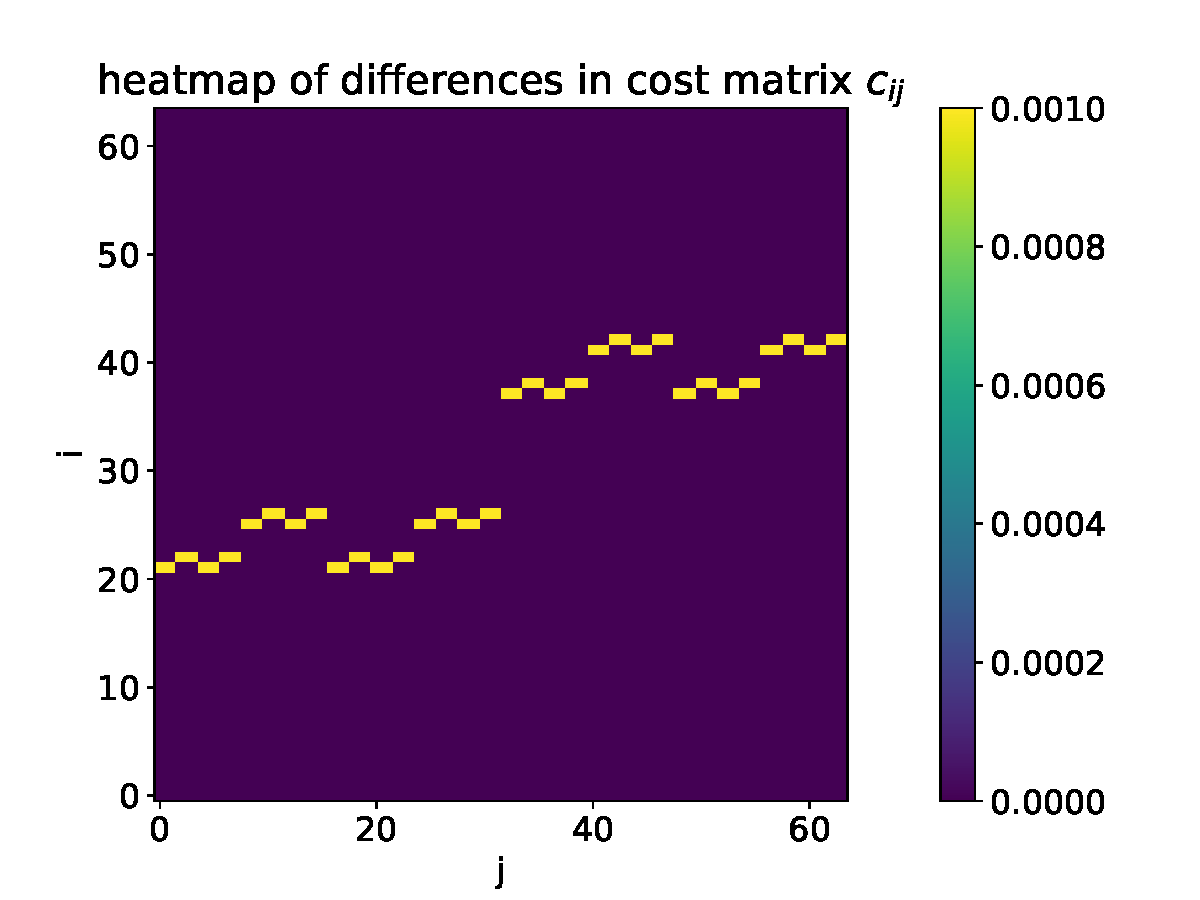
\includegraphics[width=0.5\textwidth]{./images/nonuniform_expansion_ma_n4_c-M10-exp2-newdiff.pdf}\label{fig:madiff1}}
	\subfloat[Non-uniform collapse.]{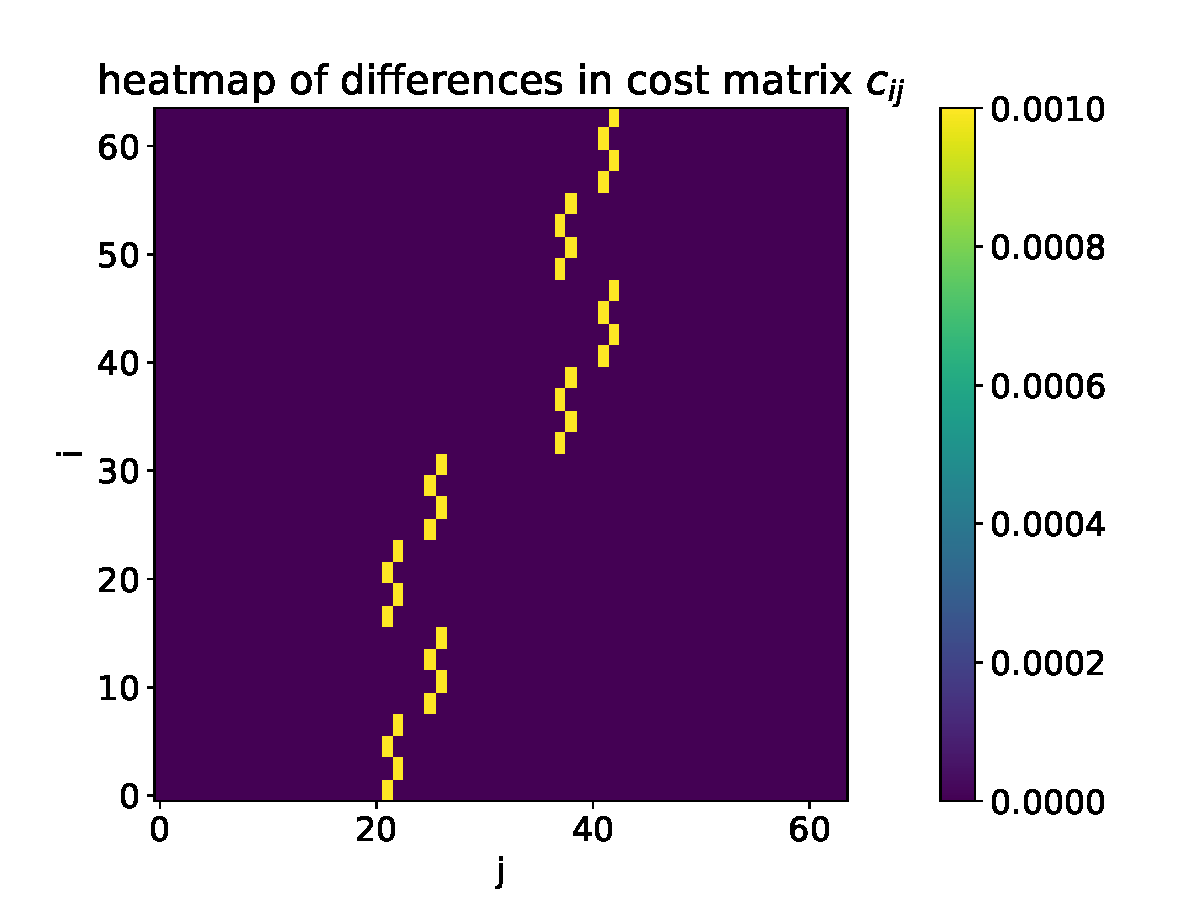
\includegraphics[width=0.5\textwidth]{./images/nonuniform_collapse_ma_n4_c-M10-exp2-newdiff.pdf}\label{fig:madiff2}}
	\caption{Heat map of the differences in the cost matrix for non-uniform expansion (left) and collapse (right) from Algorithm~\ref{alg:1} and the algorithm from \citet{ma2021}, for \lstinline|exp| $=2$ and $n = 4$.}
	\label{fig:madiff}
\end{figure}

\chapter{Additional Reference Cases}
\label{sec:apprefs}
In this appendix, we will discuss some more reference cases. Algorithm~\ref{alg:1} is used to find the cost matrix of the simulations, with $R(c) = \mathbbm{1}_U$, and $U = [0, M_c]^3$, as in Chapter~\ref{ch:results}. We choose $\gamma = \varepsilon = 1$ and $M_c = 10$. To better see differences in the heat map of the acquired cost matrix, we manually set all entries that were equal to $M_c$, equal to the highest entry of $c$ that is not equal to $M_c$. All reference cases are simulated with one million particles. In all simulations, a box size of $100$ (arbitrary units) is used. \par 
We will look at the $n=8$ case for the references for which it has not been discussed, as well as some values of \lstinline|exp| for $n=4$ which have not been discussed. 

\section{Voids}
First, we look at voids, the non-uniform expansion. All data points start in a cube centered at $(50, 50, 50)$ with sides of $50$, and particles can move towards the whole box. We simulate the same non-uniformity as in Section~\ref{sec:voids}. We look at \lstinline|exp| $=2$ and \lstinline|exp| $=5$ for $n=8$, in Figure~\ref{fig:nonuniformexpn8}. We can see some structure, but notably the \lstinline|exp| $=2$ and \lstinline|exp| $=5$ cases look structure-wise very similar; the only difference is a (not necessarily uniform) scaling. 

\begin{figure}[!ht]
	\centering 
	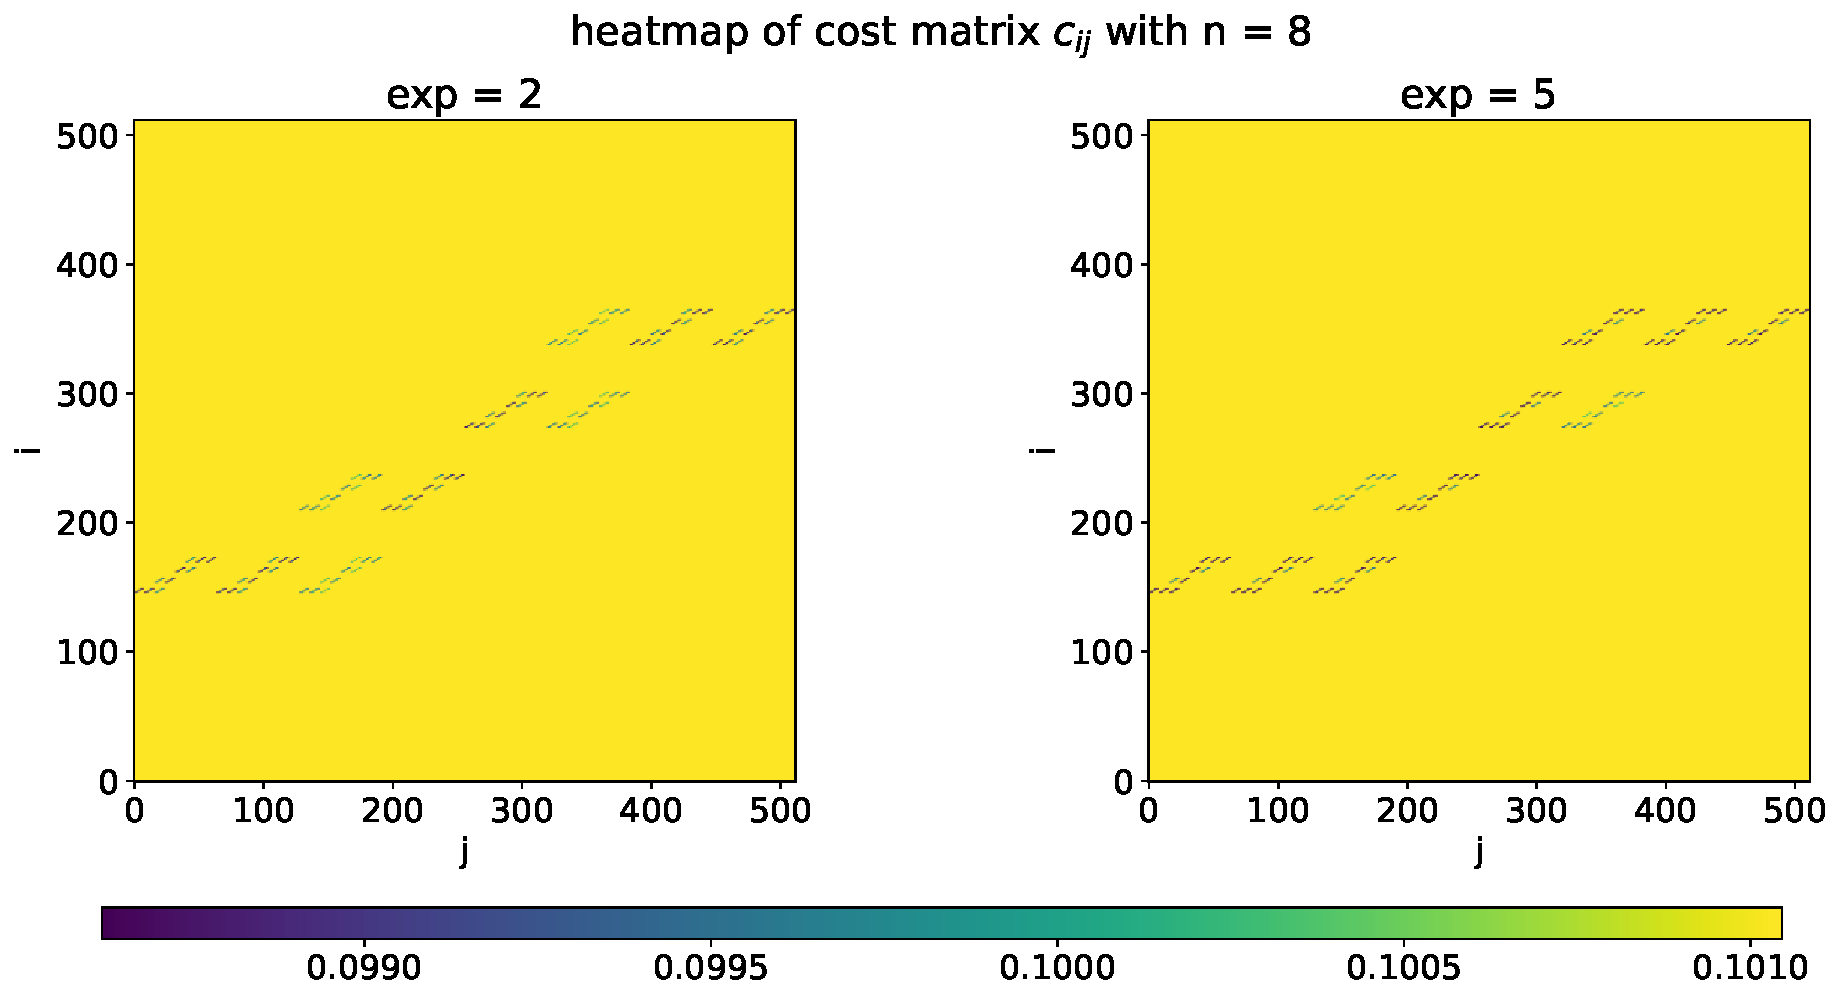
\includegraphics[width=0.8\textwidth]{./images/nonuniform_expansion_ma_n8_c-combined-exp[2, 5]-new.pdf}
	\caption{Heat map of the cost matrix for non-uniform expansion, for both \lstinline|exp| $= 2$ (left) and \lstinline|exp| $=5$ (right), for $n = 8$, as retrieved from Algorithm~\ref{alg:1}. }
	\label{fig:nonuniformexpn8}
\end{figure}

We can also look at other values of \lstinline|exp|. For example, \lstinline|exp| $= 0.4$ for $n=4$ and $n=8$, in Figure~\ref{fig:nonuniformexpn8-new}. We can see that the $n=4$ looks just like another scaling of what we already had in Figure~\ref{fig:nonuniformexpn4}, and the structure in the $n=8$ case is different, but not too different then in the \lstinline|exp| $=2$ or \lstinline|exp| $=5$ case in Figure~\ref{fig:nonuniformexpn4}. 

\begin{figure}[!ht]
	\centering 
	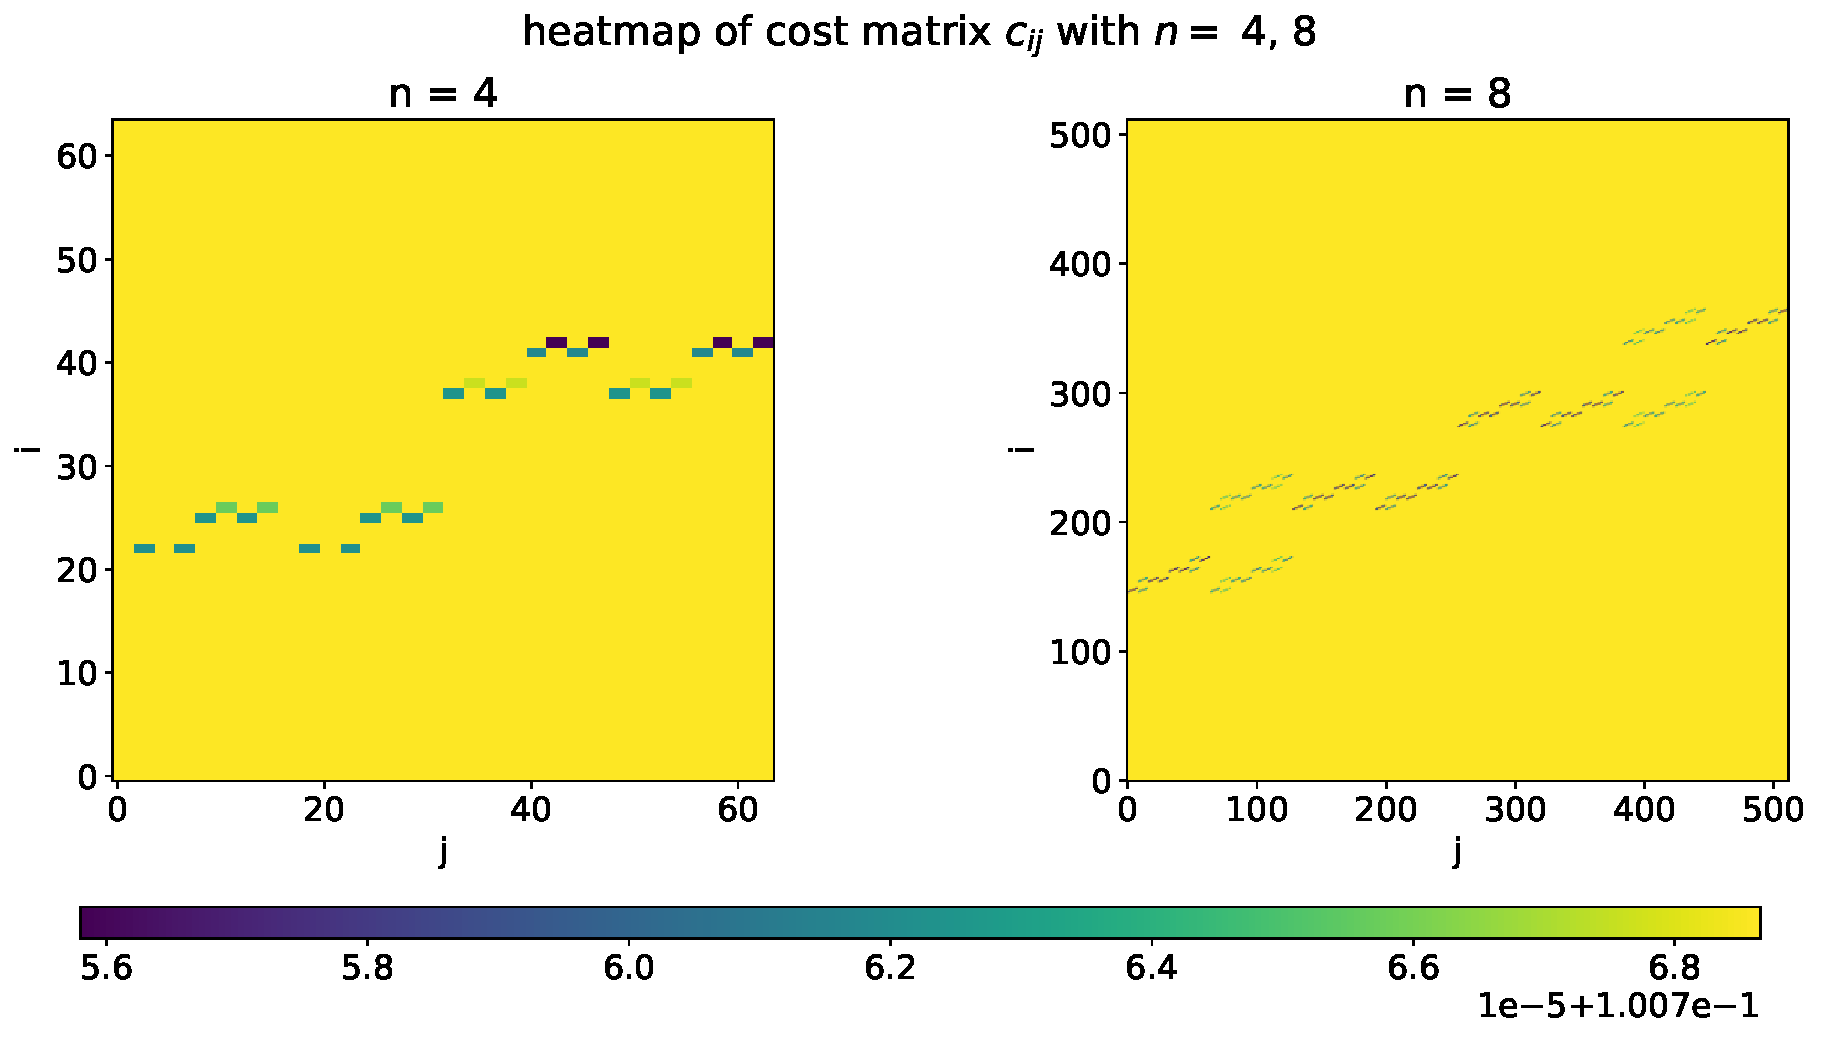
\includegraphics[width=0.8\textwidth]{./images/nonuniform_expansion_ma_ncombined-n8-new.pdf}
	\caption{Heat map of the cost matrix for non-uniform expansion, for \lstinline|exp| $= 0.4$ for both $n=4$ (left) $n=8$ (right), as retrieved from Algorithm~\ref{alg:1}. }
	\label{fig:nonuniformexpn8-new}
\end{figure}

\section{Clusters}
Let us now look at clusters, specifically at the non-uniform collapse. All data points start in the whole cube and will move towards $(50, 50, 50)$, as in Section~\ref{sec:clusters}. We look at \lstinline|exp| $=2$ and \lstinline|exp| $=5$ for $n= 8$, in Figure~\ref{fig:nonuniformcolln8}. \par 
\begin{figure}[!ht]
	\centering 
	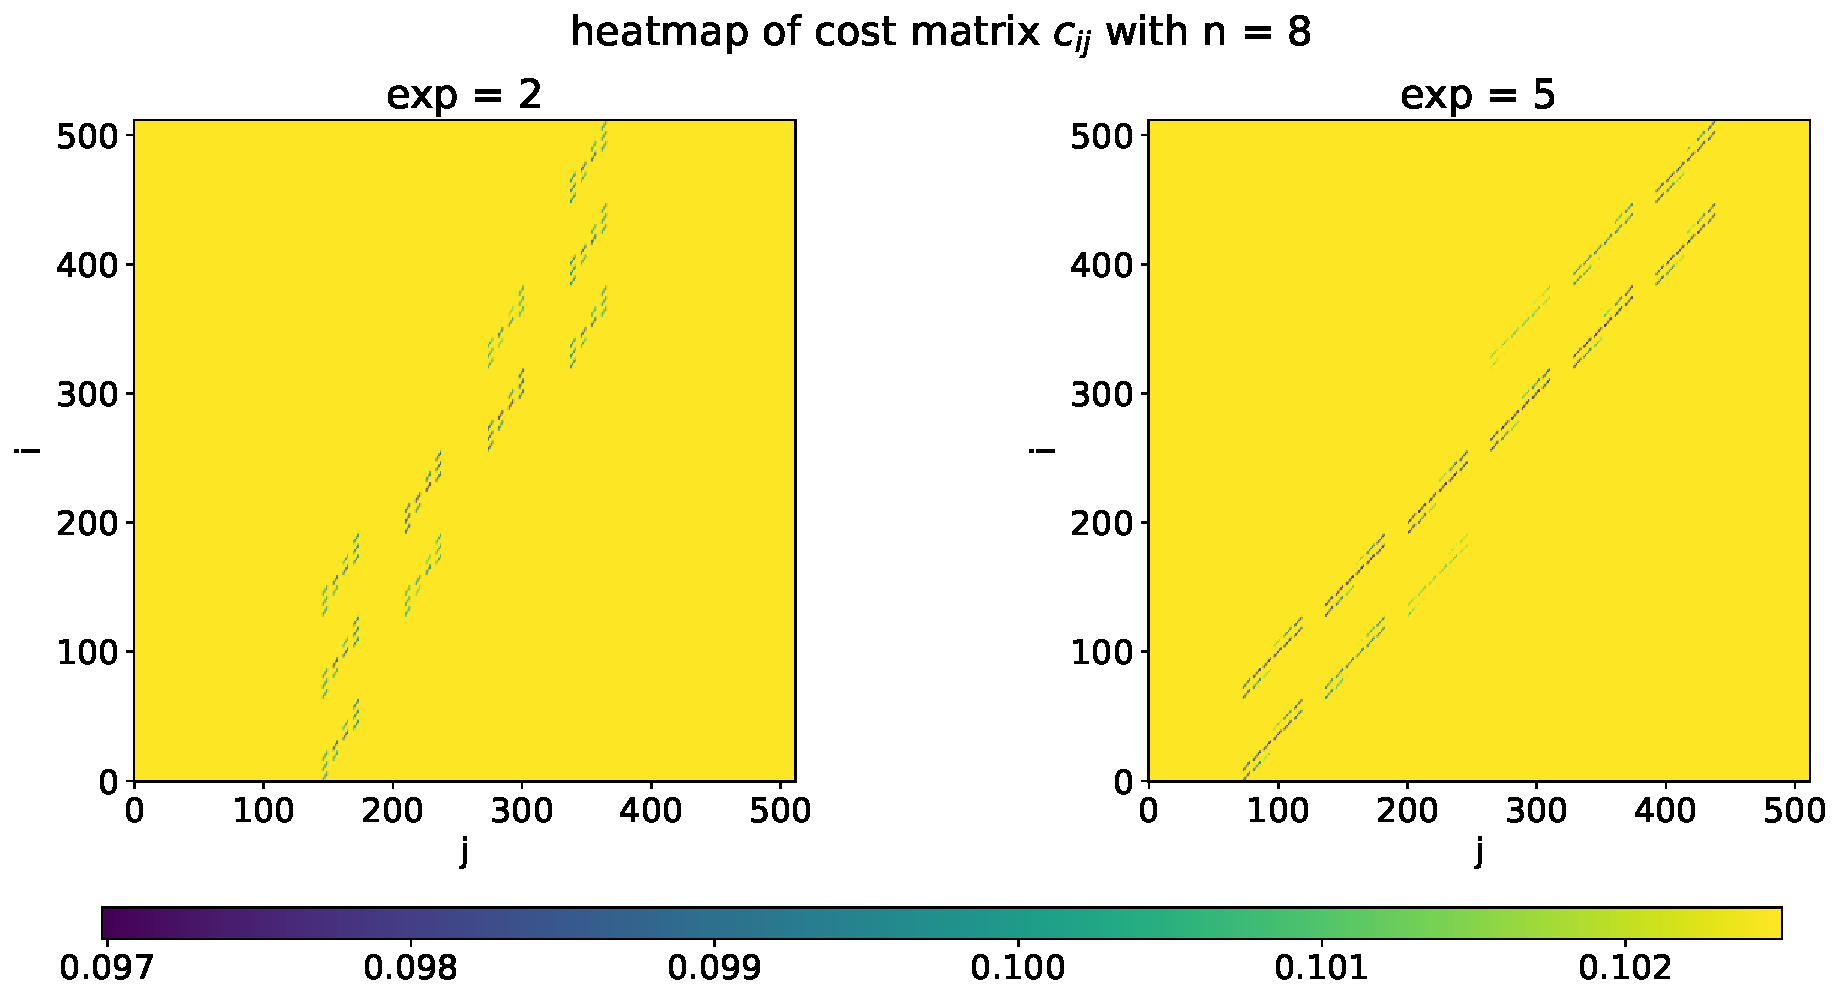
\includegraphics[width=0.8\textwidth]{./images/nonuniform_collapse_ma_n8_c-combined-exp[2, 5]-new.pdf}
	\caption{Heat map of the cost matrix for non-uniform collapse, for both \lstinline|exp| $=2$ (left) and \lstinline|exp| $=5$ (right), for $n = 8$, as retrieved from Algorithm~\ref{alg:1}. }
	\label{fig:nonuniformcolln8}
\end{figure}

In the $n=8$ case for non-uniform collapse, we can see some some structure. Note, however, that the structure is significantly different in the \lstinline|exp| $=2$ case then in the \lstinline|exp| $=5$ case. This could have been expected from the $n=4$ case in Figure~\ref{fig:nonuniformcolln4}, where for a higher value of \lstinline|exp| a more tilted structure can be seen. \par 
We can also look at other values of \lstinline|exp|. For example, \lstinline|exp| $= 0.4$ in Figure~\ref{fig:nonuniformcolln4-new} for $n=4$ and $n=8$. Note that the \lstinline|exp| $= 0.4$ case looks a lot different than any other case, especially for the higher \lstinline|exp|, for both $n=4$ as for $n=8$. This is probably due to the fact that the particle distribution changes as \lstinline|exp| grows. \par 
\begin{figure}[!ht]
	\centering 
	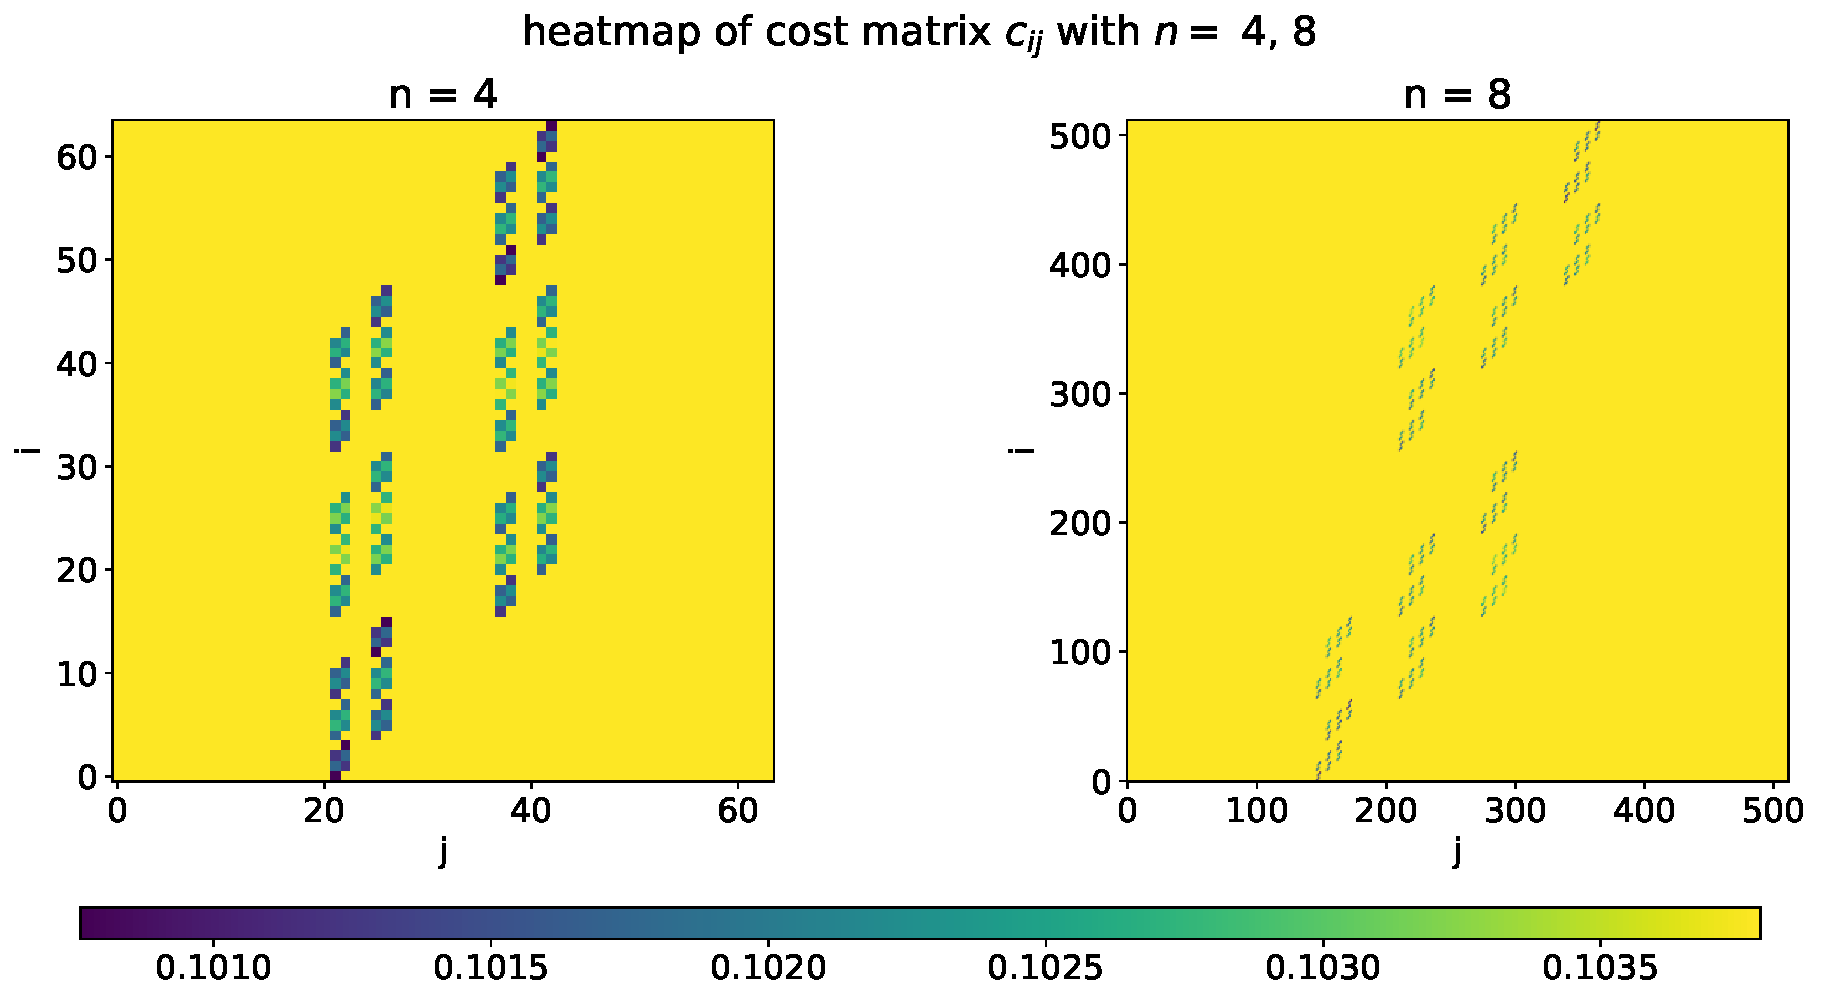
\includegraphics[width=0.8\textwidth]{./images/nonuniform_collapse_ma_ncombined-n8-new.pdf}
	\caption{Heat map of the cost matrix for non-uniform collapse, for \lstinline|exp| $=0.4$, for both $n=4$ (left) and $n=8$ (right), as retrieved from Algorithm~\ref{alg:1}. }
	\label{fig:nonuniformcolln4-new}
\end{figure}

 
\section{Walls and Filaments}
More cases of combinations of expansion and collapse, walls and filaments, were simulated too. All particles start in a cube of length $50$ and can move towards the whole box (of length $100$), as in Section~\ref{sec:refs}. For walls, the cost matrix was calculated for $n=8$, with \lstinline|exp| $=2$ and \lstinline|exp| $=5$, as can be seen in Figure~\ref{fig:walln8}. Notably the \lstinline|exp| $=2$ and the \lstinline|exp| $=5$ do not seem to differ a lot apart from a scaling. \par 
\begin{figure}[!ht]
	\centering 
	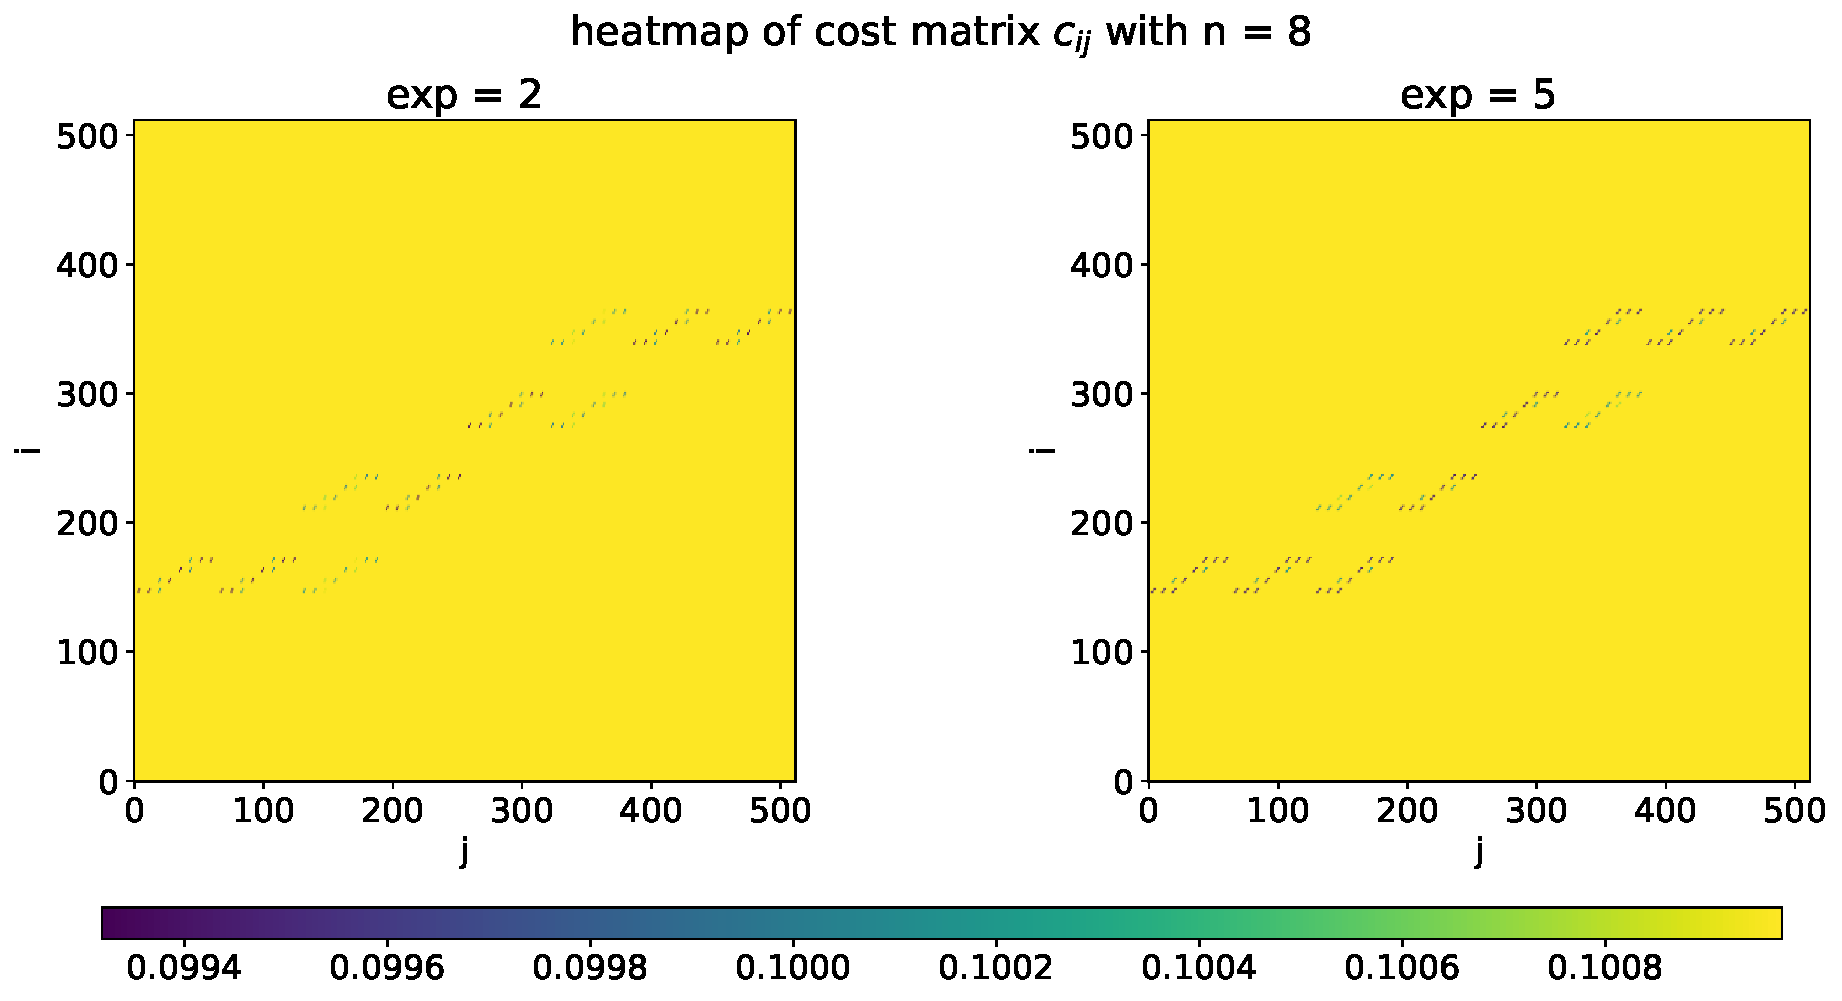
\includegraphics[width=0.8\textwidth]{./images/walls_ma_n8_c-combined-exp[2, 5]-new.pdf}
	\caption{Heat map of the cost matrix for non-uniform collapse, for both \lstinline|exp| $=2$ (left) and \lstinline|exp| $=5$ (right), for $n = 8$, as retrieved from Algorithm~\ref{alg:1}. }
	\label{fig:walln8}
\end{figure}

For filaments, the cost matrix was also calculated for $n=8$, with \lstinline|exp| $=2$ and \lstinline|exp| $=5$, as can be seen in Figure~\ref{fig:filamentn8}. In contrast to the walls, the \lstinline|exp| $=2$ case does look different than the \lstinline|exp| $=5$ case, by a rotation and a lack of some non-$M_c$ entries.
\begin{figure}[!ht]
	\centering
	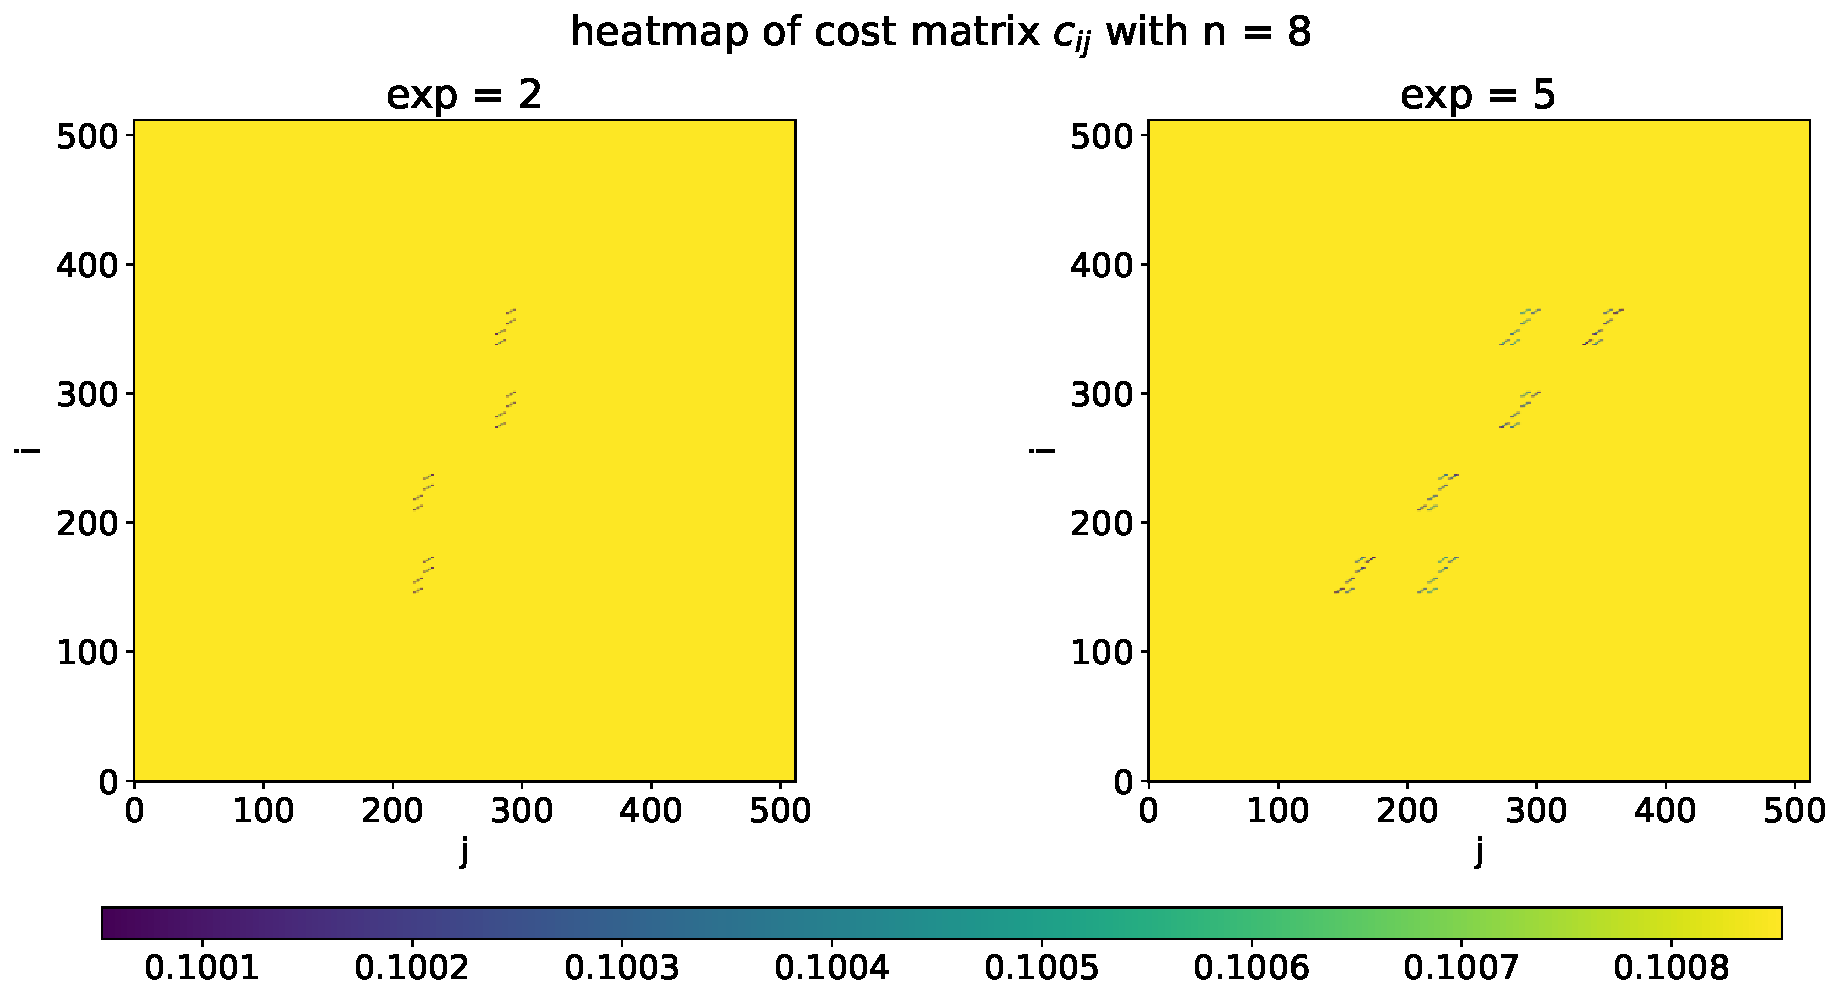
\includegraphics[width=0.8\textwidth]{./images/filament_ma_n8_c-combined-exp[2, 5]-new.pdf}
	\caption{Heat map of the cost matrix for non-uniform collapse, for both \lstinline|exp| $=2$ (left) and \lstinline|exp| $=5$ (right), for $n = 8$, as retrieved from Algorithm~\ref{alg:1}. }
	\label{fig:filamentn8}
\end{figure}




%\chapter[Markov Chain Monte Carlo Simulation Results]{Markov Chain Monte Carlo\\ Simulation Results}

%\chapter{Differences Between $\pihat$ and $c$}



